\documentclass[11pt]{article}

\usepackage{xcolor}
\usepackage{caption}
\usepackage{amsmath}
\usepackage{graphicx}
\usepackage{hyperref}
\usepackage{tabularx}
\usepackage{listings}
\usepackage{tcolorbox}
\usepackage[utf8]{inputenc}
\usepackage[margin=20mm]{geometry}

\definecolor{codegreen}{rgb}{0,0.6,0}
\definecolor{codegray}{rgb}{0.5,0.5,0.5}
\definecolor{codepurple}{rgb}{0.58,0,0.82}

\lstdefinestyle{simplecode}{
    commentstyle=\color{codegreen},
    keywordstyle=\color{magenta},
    numberstyle=\tiny\color{codegray},
    stringstyle=\color{codepurple},
    basicstyle=\ttfamily\footnotesize,
    breakatwhitespace=false,         
    breaklines=true,                 
    captionpos=b,                    
    keepspaces=true,                 
    %numbers=left,                    
    numbersep=5pt,                  
    showspaces=false,                
    showstringspaces=false,
    showtabs=false,                  
    tabsize=2
}

\lstset{style=simplecode}


% ----- END OF PREAMBLE -----




\title{Real-Time Scheduling: Project Report}
\author{Sampreet Sarkar\footnote{M2 Control and Robotics: Embedded Real-Time Systems, \textit{\'Ecole Centrale de Nantes}}}
\date{}

\begin{document}
\nocite{*}
\maketitle

\section{Introduction}
The goal of this project is to simulate the behaviour of a Preemptive Fixed-Priority Scheduler\textit{(Rate Monotonic)}. We shall move along with the assumption that all the tasks are periodic, with the task deadline equal to the task period. The design of the software will be detailed in the following sections, along with the accompanying source code, which can be found in the appendix.\\

A scheduler is an extremely important part of any Operating System, as it is in charge of breaking up tasks into jobs and executing them in a particular order to maintain the illusion of pseudo-parallelism that we commonly associate with the term \texttt{"multitasking"}. This behaviour becomes doubly important in the case of a Real-Time Operating System, because in addition to executing tasks correctly, the scheduler has to also keep in mind to return results on time, otherwise the result of the computation is invalid, and cannot be used for any good purpose.\\

Before we begin to describe the common functionalities and the design of the software, it is imperative that we take a look into the programming paradigm being followed in the development of the scheduler. The core of the scheduler has been implemented in the C++ language, which although is a close second choice of language for developping embedded applications, provides a fast enough speed and above all, embodies the use of STL classes and Object-Oriented Programming benefits. The STL template classes \textit{(especially vector and algorithm)} provide us with many helper functions, which make our life easier. Another choice to justify C++ as the optimal language of choice for this particular project is due to the innumerable open-sourced libraries that are available for the language, which lets the user accomplish a lot of complicated programming in a matter of minutes. The final executables are generated by the GNU Make\cite{make} tool, which allows us to automate the build process and give our software a little more polish. The version control is done using Git, and the online repository for the project can be found \href{https://github.com/sampreets3/scheduler-RM}{here}.\\

In the upcoming sections, we will discuss four main aspects of a scheduler|\textit{viz.}, data acquisiton, schedulability analysis, simulation of the schedule, and evaluation of the metrics. The \texttt{data acquisition} section will deal with the general idea of how to represent the contents of a simulated task to our scheduler, the \texttt{schedulability analysis} will deal with running several schedulability tests on the set of tasks in order to determine whether a given taskset is indeed schedulable or not, the \texttt{simulation} of the schedule would ideally include some representation of how the scheduling algorithm places jobs at each time instant, and the \texttt{metrics} we would want to evaluate will give us a benchmark to compare the performance of our algorithm against other solutions. Some of the metrics that define the efficiency of a scheduler is the number of context switches, the maximum idle time for the processor, and the average response time for each task.

\section{Data Acquisition}\label{sec:data-acquisition}

In this section, we are interested in obtaining the data from a simulated task, and generating our taskset $\tau$ from this data. If we think in terms of the \textit{(simulated)}scheduler, the only information we need about a task are its identifier, the computation time, the period, and the deadline of the task. Since it has already been established that in our case, the period is equal to the deadline, we can make do with either information. We also understand that we would need some kind of data structure to contain this information in an easily-retrievable fashion. Thus, we can utilize a data structure as shown in Fig. \ref{fig:tcb} below:

\begin{figure}[h!]
  \centering
  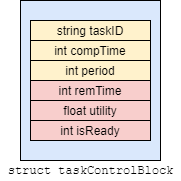
\includegraphics[scale=0.5]{../imgs/single-tcb}
  \caption{Data structure of a single task control block}
  \label{fig:tcb}
\end{figure}

We also notice that we have some extra fields in our data structure, namely \texttt{remTime}, \texttt{utility}, and \texttt{isReady}. These are not assigned by the user, but are really important to carry out the scheduling of the taskset. Here, the variable remTime stores the remaining execution time of the task, utility stores the utility of the task, and isReady is a flag that denotes the state of the task.\\

With all this information at hand, we can go ahead and create our data structure as denoted in the code listing  below. In order to increase readability, we have distributed the entirety of the code into specialised header and source files, each of which provide some special functionality to the entire software. As a result of this distributed approach, one would find it extremely easy to navigate through specific section of code, to better understand the functionality or to modify it according to the development need.

\lstinputlisting[language=c, firstline=6, lastline=16]{../../lib/tasks.hpp}

You will also observe that we have created a vector of these data structures, so that when a new task is created, the equiavalent taskControlBlock can be pushed into this vector. This will allow us to perform various vector based operations on the taskset\textit{(sorting, pushing at the tail, getting the size)} which have already been defined in the C++ STL \texttt{<vector>}.\\

Moving forward, we would like to facilitate the user's process of creating a task. For this purpose, we propose the function \texttt{createTask()}, which will allow us to create a new taskControlBlock element, and push it into the list of tasks. The implementation of the function can be seen in the following code listing\footnote{The main inspiration behind the nomenclature of the functions has been Trampoline, as it is a very elegantly designed RTOS, and since we already had some prior exposure to the functionalities.}:

\lstinputlisting[language=c, firstline=10, lastline=21]{../../src/tasks.cpp}

We have thus been able to devise a way for the user to define a task to be scheduled. Note that unlike other Fixed-Priority schedulers, we do not ask for a priority level from the user, we get around this by simply taking the size of the taskset as the maximum priority level, and ordering our taskControlBlock elements within the vector in ascending order of period. This saves us from having to validate user input, and lets us abstract the concept of priority assignment from the user.\\

In the upcoming section, we will focus on performing rigorous schedulability tests on a populated taskset, and let the user know if the schedule is indeed feasible or not.

\section{Schedulability Analysis}\label{sec:sched-analysis}

Our goal in this section is to provide an insight to the feasability of a taskset. In order to do this, we must understand the conditions for schedulability of a taskset, laid out by Liu and Layland\cite{liu-layland}. There are two conditions, the sufficient condition and the necessary condition.

\section{Simulation Results}\label{sec:sim-results}
The scheduled task set will be simulated from time zero to the first hyperperiod of the task set.
\section{Evaluation of Main Metrics}\label{sec:main-metrics}
Important metrics will be displayed. This includes the average response time of each task, the average waiting time, the time of the first deadline miss if any, etc.

\bibliographystyle{unsrt}
\bibliography{references.bib}

\section*{Appendix}

\end{document}
